\subsection{Second point}
\label{ssec:2S}

\par In this point, the goal is to simulate the operating point for $v_s(0)=0$. In order to accomplish this, we replaced the capacitor with a voltage source $V_x=V(6)-V(8)$, where $V(6)$ and $V(8)$ are the voltages in nodes 6 and 8, respectively, found in point 1. This step is, as explained in subsection \ref{ssec:2T}, based on Thévenin's theorem: we replace the capacitor with $V_s$, then we analyse all node voltages and branch currents; then, knowing $V(6)$, $V(8)$ and $I_x$, we can determine $R_{eq}$ ($R_{eq}=\frac{V_x}{I_x}$), and compute the circuit's time constant ($\tau = R_{eq}C$).
\par The results output by Ngspice are presented in the following table.

\vspace{5mm}
\begin{table}[H]
\centering
\begin{tabularx}{0.6\textwidth} {
  | >{\raggedright\arraybackslash}X
  | >{\raggedleft\arraybackslash}X | }
 \hline
@gb[i] & 4.201237e-18\\ \hline
@r1[i] & -4.01237e-18\\ \hline
@r2[i] & 4.201237e-18\\ \hline
@r3[i] & 1.888621e-19\\ \hline
@r4[i] & 8.601648e-19\\ \hline
@r5[i] & -2.84056e-03\\ \hline
@r6[i] & 8.673617e-19\\ \hline
@r7[i] & 1.700699e-18\\ \hline
v(1) & 0.000000e+00\\ \hline
v(2) & 4.139615e-15\\ \hline
v(3) & 1.270791e-14\\ \hline
v(5) & 3.552714e-15\\ \hline
v(6) & 8.589413e+00\\ \hline
v(7) & -1.78444e-15\\ \hline
v(8) & -3.55271e-15\\ \hline
v(9) & -1.78444e-15\\ \hline

\end{tabularx}
\end{table}
\vspace{5mm}

\par Comparing the simulation with the theoretical prediction, we can compute the error associated to each value. The error values are presented in the table bellow.

\vspace{5mm}
\begin{table}[H]
\centering
\begin{tabularx}{0.6\textwidth} {
  | >{\raggedright\arraybackslash}X
  | >{\raggedleft\arraybackslash}X | }
 \hline
\input{../sim/erros2_tab}
\end{tabularx}
\end{table}
\vspace{5mm}

\subsection{Third Point}
\label{ssec:3S}

\par In this point, the objective is to simulate the natural response of the circuit in node 6 for $t \in[0;20]$ms, that is, the evolution of this node's voltage throught time, when all independent sources are switched off. As the used boundary condition is $V(6)$ and $V(8)$ equal to the values found in point \ref{ssec:2S} for this nodes, we used the command \textit{.include} in the \textit{Ngspice's} script so that this values are imported automatically.
\par The obtained result is plotted bellow.

\begin{figure}[h] \centering
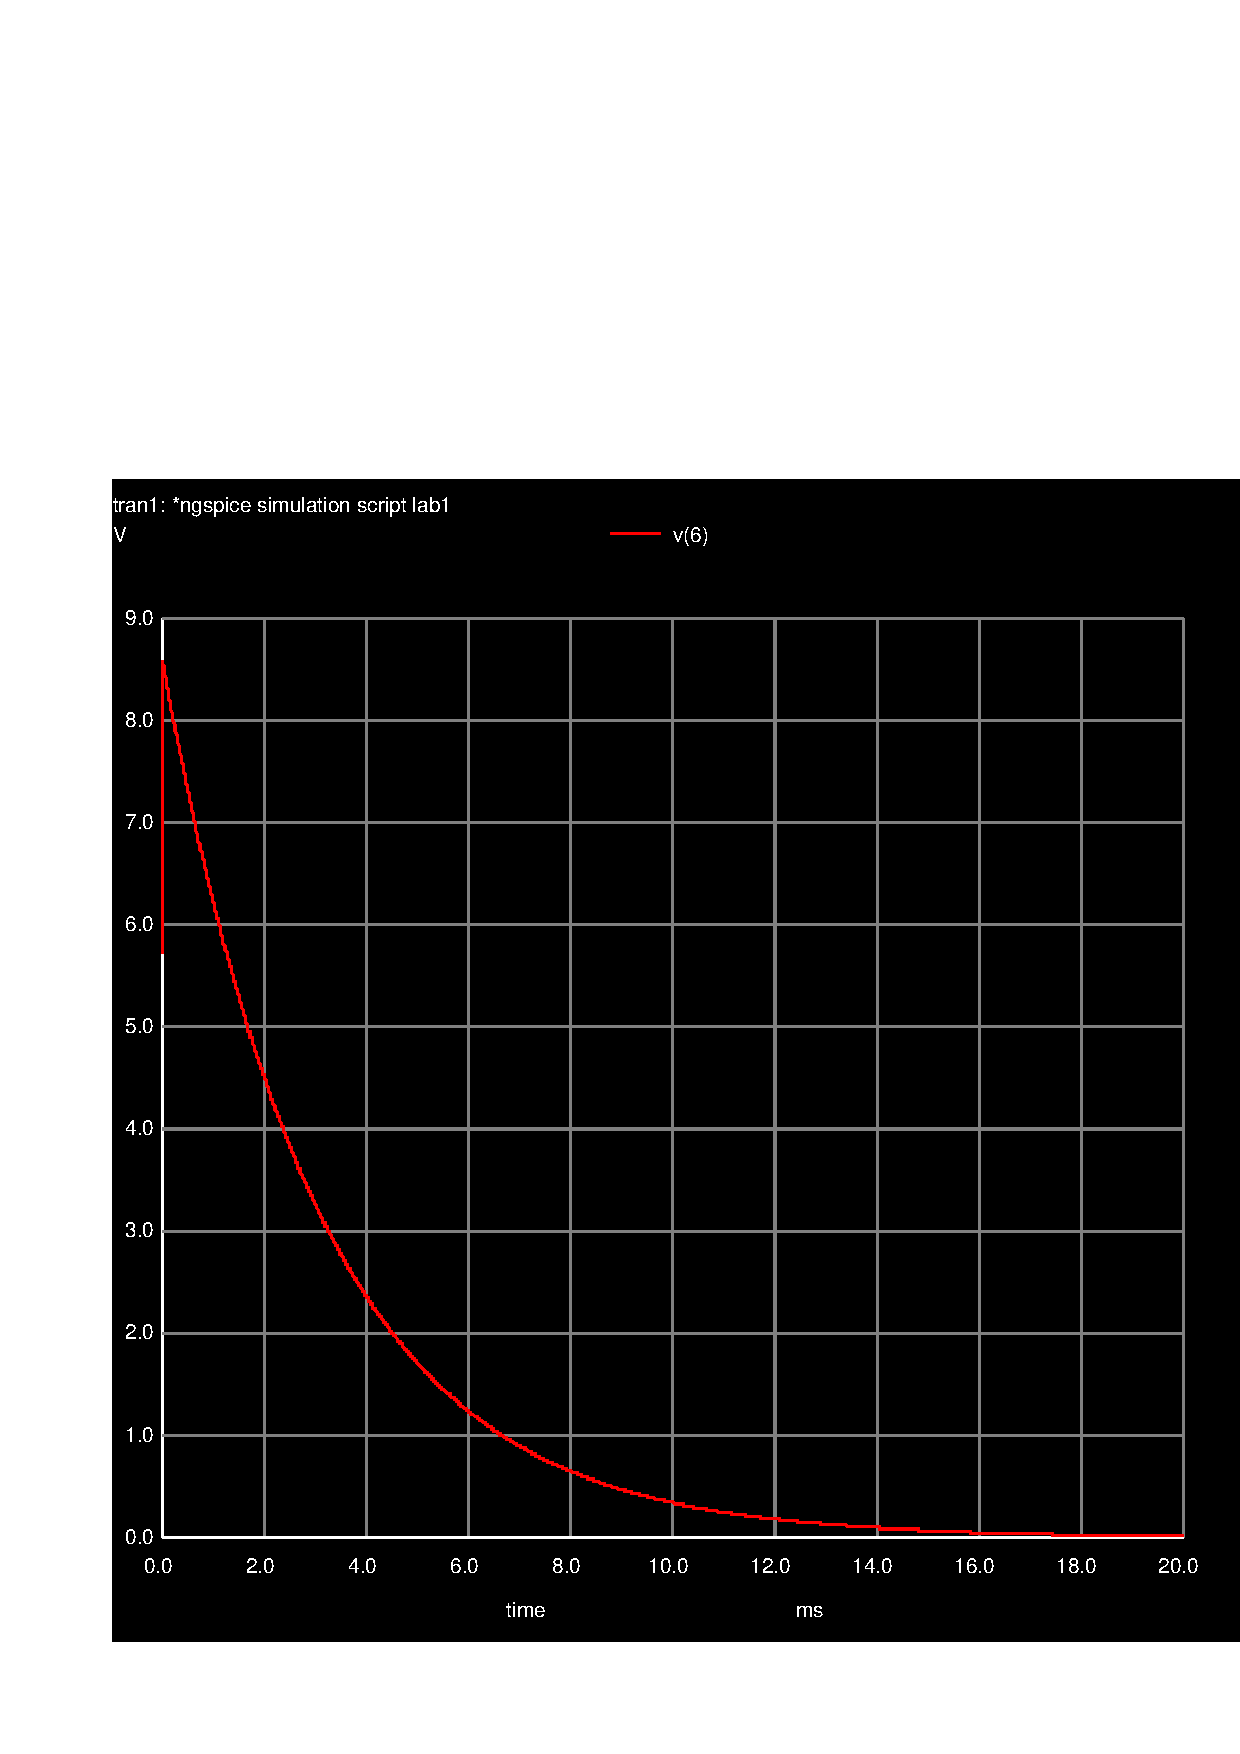
\includegraphics[width=0.7\linewidth]{../sim/teste_3.pdf}
\caption{Natural solution $v_{6n}(t)$, $t\in[0,20]$ms (simulation)}
\label{fig:snat_sim}
\end{figure}
